\chapter{RosettaHTS: A virtual High Throughput Screening tool integrating structure and ligand based information}
\label{chap:rosetta_hts}
\section{Introduction}

\subsection{Ligand docking methods are inconsistently able to predict binding affinity}

While protein-ligand docking tools are frequently capable of correctly predicting poses\citep{Trott:2010km,Friesner:2004hm,Ewing:2001wu}, these methods have proven limited in their ability to distinguish between active and inactive compounds\citep{Bauer:2013de,Huang:2006gi,Davis:2009fx}.
The DEKOIS 2.0 benchmark published in 2013 \citep{Bauer:2013de} and a blind study of protein-ligand docking tools conducted in 2009\citep{Davis:2009fx} demonstrated that the majority of protein-targets can successfully be studied with protein-ligand docking tools, although the tool with the best performance varies based on the target.
This suggests that protein-ligand docking as a broad class of technique generally has the ability to be successful. 
However, the overall variance in ligand docking performance suggests that while active and inactive ligands can be classified for most protein systems by at least one available tool, no tool is universally reliable.
Furthermore, it has not been possible to easily predict which protein systems can be successfully targeted by which by which ligand docking tools. 

\subsection{Neural Network based methods can be used to re-score protein-ligand binding prediction}

In recent years, several tools have been developed to re-score protein-ligand binding predictions using neural networks.
NNScore\citep{Durrant:2010js} and NNScore\citep{Durrant:2011dx} are two such tools.
A benchmark of neural network based scoring methods published in 2013 suggested that while these methods are frequently capable of improving activity classification and binding affinity prediction beyond protein-ligand docking, the success of the method remains highly dependent on protein target.\citep{Durrant:2013db}

\subsection{Existing limitations in training data sources}

\subsubsection{The limitations of existing sources of active ligands}
As the goal of RosettaHTS was to train a model capable of distinguishing between active and inactive small molecules across a range of protein targets and small molecule chemical space, the selection of a high quality training set was crucial.
There are several factors which complicate the selection of a training set for a general classifier.
First, compounds with known binding affinity must be located across a wide range of protein targets.
Because the goal is to compare ligands independent of protein target, \ki\ must be used rather than \ic.
This substantially reduces the availability of data from public databased such as ChEMBL or PubChem. 
Furthermore, the active compounds selected must bind to a wide and evenly distributed range of targets, and have a wide and evenly distributed range of known activities.
Due to the realities of the drug discovery process, neither publicly nor privately available compound databases meet these requirements.
For example, while ChEMBL contains 481050 \ki\ value measurements across 164 distinct targets with known \ki values, 90\% of these targets have fewer than 891 measurements each.
In other words, nearly all of the available \ki\ values are confined to a small handful of protein targets.

\subsubsection{The limitations of existing sources of inactive ligands}
The difficulty of selecting a high quality training dataset is compounded by the availability of known inactive ligands. 
The activity data of inactive ligands is less frequently published than active ligands.
Additionally, most inactive ligands are measured as inactive by \ic\ rather than \ki.
Because \ic\ and \ki are distinct properties, a compound with no measurable \ic\ cannot necessarily be said to have no measurable binding affinity.

\subsubsection{Property matching schemes used for ligand docking benchmarks are not sufficient for training purposes}
The above-mentioned issue of the lack of known inactive compounds is frequently addressed by the use of property matching.
In this process, compounds that have similar chemical properties to the known active ligands but dissimilar structures are selected and designated as presumed inactive compounds\citep{Huang:2006gi, Mysinger:2012hu, Bauer:2013de}.
This property matching scheme can be useful for the benchmarking of ligand docking methods, but cannot be used as the basis of training data sets for machine learning techniques.
Because the property matching scheme is algorithmically selecting ligands in a slightly different part of chemical space compared to the known active ligands, the risk exists of the neural network learning to classify ligands based not on their binding affinity but rather the property matching scheme used to select them.

\section{Results}

\subsection{Development of a balanced training dataset}
\label{subsec:dataset_description}

\subsubsection{Cross-docking a diverse set of ligands to create a balanced set of training data}
\label{subsubsec:pdbbind_overview}
A cross docking approach is used to create the training dataset.
PDBBind\citep{Wang:2004cm} is a collection of Protein-ligand binding pairs for which known binding affinities and X-ray crystal structures exist.
Since it's original publication in 2004, The PDBBind database has been periodically updated, and as of 2013, contains 10776 total complexes, of which 2959 have known \ki\ values, are non-covalently bound, have only a single ligand in the binding site,  and have crystal structures with a resolution of less than 2.5 \AA.
Compounds from this "refined" subset of the PDBBind database were used as the basis of the training dataset.

\subsubsection{Additional filtering of PDBBind "refined" to produce a diverse set of high quality active compounds}
\label{subsubsec:active_poses}
For the purposes of this training set, all active ligands must have the following properties beyond those described in section \ref{subsubsec:pdbbind_overview}:
The set of proteins must be diverse, every protein in the set should come from a different family to avoid biasing training.
While RosettaLigand is capable of docking ligands into proteins into ligands of any side, extremely large proteins require the allocation of large amounts of memory, which makes screening more time consuming.
As a result, all proteins in the training set should have <1000 total residues across all chains.
RosettaLigand must be capable of predicting the pose of each complex such that the lowest Rosetta score has an \ac{RMSD} of < 2.0 \AA\ to the crystal structure.
the 2959 complexes in the PDBBind refined set were filtered based on the first two criteria, and then docked using the RosettaLigand protocol described in chapter \ref{chap:lowres_paper}, resulting in a set of 507 unique protein-ligand complexes (Table \ref{table:training_pdbs}. 
This set of compounds is very diverse in chemical space, ranging from small fragments to small peptides, with the bulk of the distribution consisting of small drug-like molecules.
Specifically, the number of atoms ranges from 6 to 171, with a median of 44, the number of rings ranges from 0 to 8 with a median of 2. The number of rotatable bonds ranges from 0 to 49 with a median of 6, and the weight ranges from 87.06 to 1107.58 with a median of 107.
Figure \ref{fig:training_ligands} shows histograms of these plots.
The large diversity of this training set is desirable, as the goal is to produce a model with as wide an applicability domain as possible.

\begin{figure}
\centering
\includegraphics[width=4in]{figures/hts/basic_ligand_properties.pdf}
\caption{
The basic property distribution of ligands in the training data set.  Histograms are plotted of the atom count, rotatable bond count, ring count, Topological Polar Surface area, log(\ki) and molecular weight of the 507 ligands in the binding site. 
}
\label{fig:training_ligands}
\end{figure}
\begin{table}
\scriptsize
\renewcommand{\tabcolsep}{0.09cm}
\centering
\begin{tabular}{|c|c|c|c|c|c|c|c|c|c|c|c|c|}
\hline
2glp & 1m7y & 2v7d & 3nkx & 4f7v & 2am4 & 2gzl & 3ery & 2buv & 4b0b & 2vba & 1x8r & 1k1y \\
\hline
1k27 & 1q91 & 2e7f & 1kyv & 2c92 & 2c94 & 1ex8 & 1pgp & 3tfu & 3ldp & 1h2t & 2vk2 & 3k00 \\
\hline
1w96 & 1gpk & 2ybu & 3eqr & 2fxu & 3eks & 2jkh & 3b92 & 1add & 2i6b & 1wc1 & 1ch8 & 1ua4 \\
\hline
1efy & 1fzq & 1ws4 & 2wzm & 1y3p & 1ppi & 2pmk & 3f6g & 2zxg & 2xb7 & 3rf5 & 1xow & 1j36 \\
\hline
3qqs & 3m3c & 1a4k & 3s0b & 3kiv & 2aac & 2q7q & 1t5f & 3lp7 & 2hjb & 2hw2 & 3ip8 & 3pwk \\
\hline
3k4q & 1qji & 2cgf & 1atl & 3uod & 1lrh & 2a5c & 3lbz & 2qmg & 1ft7 & 2vsl & 3qkd & 1x38 \\
\hline
1oif & 3sus & 1i5r & 1pzo & 2vl4 & 1hp5 & 1z4o & 2fdp & 1bju & 3v7t & 2v58 & 3cm2 & 3rux \\
\hline
2dw7 & 1fl3 & 3c88 & 3nq3 & 3lk1 & 2wp1 & 1wn6 & 2vvn & 2oiq & 3bxh & 3odu & 3sxf & 3uuo \\
\hline
3rdv & 3t1m & 2bes & 3eft & 3pgl & 1cbx & 1m2p & 3ui7 & 3l0v & 3i4y & 1lyb & 2zdk & 3dnj \\
\hline
2q7y & 1jsv & 4agl & 4f9u & 2r0h & 2pv1 & 1n8v & 1i7z & 1c5c & 1w9u & 1t31 & 3n7o & 4dkp \\
\hline
1utc & 4f20 & 3qps & 2b7d & 1z6e & 966c & 2v95 & 2zcq & 3gxy & 3pju & 1pxn & 1ctt & 2i80 \\
\hline
2vvp & 2pql & 2zy1 & 2y8c & 2o1c & 1laf & 1dhi & 3cyz & 2vmd & 1kzn & 1nw5 & 2cc7 & 2yay \\
\hline
3dvp & 2pq9 & 4erf & 1i8i & 1ela & 3nyd & 1h5v & 2oym & 1epo & 3dsz & 1ebg & 1xkk & 2we3 \\
\hline
1ikt & 3g3r & 2ydt & 3hp9 & 1xk9 & 3lka & 2r1y & 2jg0 & 2i19 & 1hmr & 1qft & 2wjg & 4b8y \\
\hline
4auy & 3hv8 & 3ies & 2hah & 3lc3 & 1d7i & 1nki & 2hzy & 1a4r & 2o4s & 3su0 & 3a5y & 1n7m \\
\hline
3qyy & 4ad2 & 1gai & 2j47 & 2v3d & 2wzf & 2afw & 1ydk & 1c2t & 1r9l & 1q5k & 2euk & 2wvt \\
\hline
4a95 & 2vo4 & 2qt5 & 3e3c & 1jyq & 3gx0 & 1fo0 & 3bl0 & 3hkw & 3m3z & 3upv & 1nhu & 1r0p \\
\hline
1hsl & 3mz6 & 4ek9 & 1d4h & 3qfd & 3b7j & 2vpe & 1r6n & 2xab & 2uxi & 2j4g & 5yas & 1gyx \\
\hline
1x8d & 1bzy & 3ozg & 2q6f & 2vnp & 1yei & 1jgl & 2c1p & 3bft & 3miy & 4ewn & 2pcp & 3q5u \\
\hline
1lbf & 1rd4 & 1m48 & 3rv8 & 1grp & 1jzs & 1q54 & 3uxd & 1zhy & 2ojg & 1qin & 1ax0 & 1yqy \\
\hline
3bze & 2r59 & 3f8c & 3aaq & 3i9g & 3f78 & 1lst & 1lgw & 2y7k & 3imc & 3ebi & 2e7l & 2hu6 \\
\hline
1gcz & 3fj7 & 2v25 & 1qy2 & 1ez9 & 3uxk & 2haw & 3g0e & 1mmq & 3f15 & 1jao & 3u15 & 2vkm \\
\hline
2fqw & 3iog & 1kug & 1pfu & 1ik4 & 3qt6 & 2oi2 & 3qx8 & 2gj5 & 2ojj & 3gt9 & 3kek & 3dzt \\
\hline
3g08 & 3hmp & 1jys & 3a6t & 3iob & 1e6q & 3p8p & 1gwv & 3tg5 & 3ctt & 1szd & 2cia & 1r1h \\
\hline
1zs0 & 2qtn & 3bbb & 3nyx & 3p8z & 3su3 & 1n4h & 1ucn & 2w66 & 3n7h & 1b05 & 3ahn & 1duv \\
\hline
1dqx & 3td4 & 3ipq & 3hl7 & 2wyf & 2ves & 3old & 2ews & 3coy & 2qbw & 1ai4 & 1apv & 1c3x \\
\hline
2rkd & 3o84 & 1icj & 3o4k & 2itk & 3tcg & 3uug & 1fch & 3fur & 2r0z & 3b4p & 3sk2 & 1hnn \\
\hline
3p7i & 2o8h & 3uj9 & 1bq4 & 1fv0 & 2dua & 3k5i & 1njs & 2gvv & 3acl & 1lee & 1ceb & 2q8z \\
\hline
3bgs & 1mrw & 2p3a & 4b1j & 3kjd & 3jzg & 2d3u & 2p4y & 1rpj & 2yim & 3a1c & 3v78 & 1sr7 \\
\hline
1wm1 & 1hn4 & 2zmm & 4g0p & 1qbq & 2ylc & 2wos & 2qbp & 4sga & 3f3t & 1eoc & 3h78 & 4dhl \\
\hline
2q88 & 3ohi & 2rin & 3jrs & 1a99 & 4eoh & 1n2v & 3rdq & 3g0w & 3hvi & 3fwv & 1xap & 1x8j \\
\hline
1iiq & 1hi4 & 2xog & 1uj5 & 3f5k & 3ebl & 1br6 & 3re4 & 3sfg & 4eo6 & 2p3i & 1drj & 2fqo \\
\hline
2wuf & 3hzm & 2uy3 & 2qrl & 3hit & 2std & 1fkn & 1dfo & 2w8j & 3myg & 1nvq & 1hk4 & 1kdk \\
\hline
3o5n & 1wcq & 4aq4 & 1xk5 & 1pot & 4h75 & 3omc & 3acw & 1ogx & 1df8 & 1b8y & 2rcn & 2gv6 \\
\hline
2vuk & 3egt & 3bkk & 3kr8 & 3udd & 1ork & 1os0 & 2gh9 & 4gah & 3lqi & 2bvs & 1e2k & 1uou \\
\hline
1mrn & 1bp0 & 1n46 & 2xn3 & 3bex & 3ewj & 2ce9 & 4f5y & 1e4h & 3nee & 2hzl & 1byk & 1nli \\
\hline
2ra6 & 1amk & 4tim & 1enu & 1adl & 3hf8 & 1eb2 & 4a6l & 2fpz & 2ov4 & 4b9w & 3obq & 3nhi \\
\hline
1b55 & 2azr & 3k5v & 2nt7 & 4ts1 & 3ny3 & 3nzk & 3iss & 1upf & 1ui0 & 1w0z & 1ejn & 3pyy \\
\hline
3kgt & 2v54 & 2qu6 & 2v83 & 3gsm & 1db1 & 2h6q & 1fh8 & 3zq9 & 4ai5 & 2fxs & 2weq & 2gkl \\
\hline
\end{tabular}
\caption{The \acs{PDB} IDs of the protein-ligand complexes selected for use in the training data set.}
\label{table:training_pdbs}
\end{table}

\subsubsection{Crossdocking active compounds produces presumed inactive binding data}
The best scoring, lowest \ac{RMSD} binding poses selected in section \ref{subsubsec:active_poses} will comprise the active component of the training set.
The inactive component of the training set was generated through cross-docking.
Each ligand in the 507 compound set was docked into each of the proteins in the set except the one with measured activity data.
Due to the size of chemical space\citep{Reymond:2012un} and the diversity of the protein-ligand complexes in the dataset, it can be reasonably assumed that every cross-docked complex has no binding affinity.
The lowest scoring Rosetta model for each cross-docked complex was selected, and the resultant set of 250970 protein-ligand complexes will comprise the inactive component of the training set.

\subsection{Development and description of ligand descriptors}
\label{subsec:descriptor_development}
\subsubsection{Sources of descriptor data} 

The proper selection of descriptors is critical for the training of an effective model.
It is frequently difficult to determine \textit{a priori} which descriptors will be the most useful, so three classes of descriptor information were evaluated.  Specifically: scalar scores and statistics describing the protein-ligand interface,  \ac{RDF} descriptors describing the arrangement of atoms in the protein-ligand interface, and scalar metrics describing the ligand chemistry.

\subsubsection{Scalar protein-ligand interface descriptors}
\label{subsubsec:scalar_rosetta}
The RosettaLigand energy function directly provides a number of metrics that can be used as scalar descriptors of the chemistry of the protein-ligand interface.
In addition to these scores, Rosetta implements an "Interface Analyzer" which generates additional descriptors of the protein-ligand interface.
Between these two descriptor sources, a set of 20 descriptors can be computed, describing the van der waals, hydrogen bonding, desolvation and electrostatic energy of the protein-ligand interface, as well as the size of the protein binding pocket, the number of unsatisfied hydrogen bonds, and the \ac{SASA} of the interface.
Table \ref{table:rosetta_scalar} summarizes the specific scalar interface descriptors used.
\begin{table}
\scriptsize
\renewcommand{\tabcolsep}{0.09cm}
\centering
\begin{tabular}{|c|c|}
\hline
\textbf{Property name} & \textbf{Description} \\
\hline
\multicolumn{2}{|c|}{\textbf{Rosetta energy descriptors}} \\
\hline
if\_X\_fa\_atr & Attractive force of the protein-ligand interface\\
\hline
if\_X\_fa\_rep & Repulsive force of the protein-ligand interface\\
\hline
if\_X\_fa\_intra\_rep & Repulsive force between atoms in each residue and the ligand \\
\hline
if\_X\_fa\_elec & Electrostatic force of the protein-ligand interface \\
\hline
if\_X\_fa\_pair & The value of the Rosetta pair energy between protein and ligand residues\\
\hline
if\_X\_fa\_sol & The desolvation energy of the protein-ligand interface \\
\hline
if\_X\_hbond\_bb\_sc & The hydrogen bonding energy between protein backbone atoms and ligand atoms \\
\hline
if\_X\_hbond\_sc & The hydrogen bonding energy between protein side chain atoms and ligand atoms \\
\hline
hbond\_lr\_bb & The long range hydrogen bonding energy between protein backbone atoms in the entire complex \\
\hline
hbond\_sc & The hydrogen bonding energy between all side chain atoms in the entire complex\\
\hline
hbond\_sr\_bb &  The long range hydrogen bonding energy between protein backbone atoms in the entire complex\\
\hline
interface\_delta\_X & The total Rosetta score associated with the protein-ligand interface\\
\hline
total\_score/nres\_all & The total complex score divided by the total number of protein residues \\
\hline
\multicolumn{2}{|c|}{\textbf{Rosetta Interface Analyzer descriptors}} \\
\hline
dSASA\_hydrophobic & The hydrophobic SASA at the protein-ligand interface  \\
\hline
dSASA\_int & The total SASA at the protein-ligand interface  \\
\hline
dSASA\_polar & The polar SASA at the protein-ligand interface \\
\hline
delta\_unsatHbonds & The number of unsaturated hydrogen bonds at the protein-ligand interface\\
\hline
hbond\_E\_fraction & The fraction of the interface energy associated with hydrogen bonding\\
\hline
nres\_int & The number of protein residues at the protein-ligand interfaec\\
\hline
packstat & The protein-ligand interface packing statistic originally described by Sheffler \citep{Sheffler:2009bd} \\
\hline
\end{tabular}
\caption{A summary of the names and definitions of the scalar descriptors generated by Rosetta.
Rosetta energy descriptors were originally described by Rohl\citep{Rohl:2004dh} }
\label{table:rosetta_scalar}
\end{table}

\subsubsection{Scalar ligand descriptors}
\label{subsubsec:scalar_bcl}
The scalar descriptors discussed in section \ref{subsubsec:scalar_rosetta} encode only information related to the protein-ligand interface.
To provide information about the chemistry of the ligand, an additional set of ligand descriptors are computed using the \ac{BCL}.
These descriptors provide information about the weight of the ligand, the number of hydrogen bond donors and acceptors, predicted LogP, number of rings, number of rotatable bonds and the circumference of the ligand around the widest dimension.
Table \ref{table:bcl_scalar} summarizes the scalar ligand descriptors.
\begin{table}
\scriptsize
\renewcommand{\tabcolsep}{0.09cm}
\centering
\begin{tabular}{|c|c|}
\hline
Property name & Description \\
\hline
Weight & The molecular weight of the ligand\\
\hline
HbondDonor & The number of hydrogen bond donors in the ligand\\
\hline
HbondAcceptor & The number of hydrogenn bond acceptors in the ligand\\
\hline
LogP & The predicted logP (partition coefficient) of the ligand\\
\hline
TotalCharge & The total calculated charge of the ligand\\
\hline
NRotBond & The number of rotatable bonds of the ligand\\
\hline
NAromaticRings & The number of aromatic rings of the ligand\\
\hline
NRings & The total number of rings of the ligand\\
\hline
TopologicalPolarSurfaceArea & The topological polar surface area of the ligand\\
\hline
Girth & The circumference of the ligand around the widest dimension\\
\hline
\end{tabular}
\caption{A summary of the names and definitions of the scalar descriptors generated by the \acs{BCL}. }
\label{table:bcl_scalar}
\end{table}
The number of descriptors used to describe the ligand is relatively small compared to previous machine learning studies performed using the \ac{BCL}\citep{Mueller:2010dx}.
The rationale for including a smaller number of descriptors is that a relatively small number of ligands is being used to train the classifier.
As a result, the descriptions of the ligand chemistry used should be broad enough that the range of the descriptor space is well covered.

\subsubsection{Protein-ligand fingerprint descriptors}
In addition to the scalar descriptors  discussed in sections \ref{subsubsec:scalar_rosetta} and \ref{subsubsec:scalar_bcl}, a novel set of protein-ligand interface descriptors were added.
These fingerprint descriptors are implemented as \ac{RDF}s, which take the following form:
\begin{equation}
g(r) = \frac{1}{2}\sum_{\substack{i,j \\ i \neq j}}score_{ij}e^{-B(r-r_{ij})^{2}}
\end{equation}
Where $i$ and $j$ are a protein and ligand atom respectively, $score_{ij}$ is a score computed based on those two atoms, $B$ is a smoothing factor, $r$ is the radius of the sphere being currently considered, and $r_{ij}$ is that distance between the two atoms.
The function $g(r)$ computes the \ac{RDF} for a single distance.  To compute the complete fingerprint, $g(r)$ is computed for a range of values of of $r$.
The resulting fingerprint represents the probability of two atoms existing within a sphere of radius $r$ with some property. 
More broadly, these fingers can be interpreted as a 1 dimensional representation of the 3 dimensional distribution of geometric and chemical properties in the protein-ligand interface. 
A range of fingerprints were computed using this method, with various chemical properties used to compute $score_{ij}$.
Fingerprints are computed using the attractive, repulsive,electrostatic, solvation and hydrogen bonding scores used by Rosetta.  Additionally, a charge based function is implemented in which $score_{ij}$ is computed as the product of the charges of each atom pair, and a hydrogen bond count function is computed in which $score_{ij}$ is 1.0 if the pair of atoms are a hydrogen bond donor and acceptor, and 0.0 otherwise.
The fingerprints are computed directly by Rosetta.
Table \ref{table:rosetta_fingerprint} summarizes the \ac{RDF} fingerprints computed by Rosetta.
Based on previous experience with \ac{RDF} fingerprints in the \ac{BCL}, all fingerprints are computed using 24 evenly spaced distance steps between 0 and 6.0 \AA.
\begin{table}
\scriptsize
\renewcommand{\tabcolsep}{0.09cm}
\centering
\begin{tabular}{|c|l|}
\hline
atr\_interface\_rdf & RDF using the Rosetta attractive score between pairs of atoms\\
\hline
solv\_interface\_rdf & RDF using the Rosetta desolvation score between pairs of atoms \\
\hline
elec\_interface\_rdf & RDF using the Rosetta electrostatic score between pairs of atoms\\
\hline
rep\_interface\_rdf & RDF using the Rosetta repulsive score between pairs of atoms \\
\hline
hbond\_acceptor\_interface\_rdf & RDF using the Rosetta hydrogen bonding term between ligand acceptor atoms and protein donors\\
\hline
hbond\_donor\_interface\_rdf & RDF using the Rosetta hydrogen bonding term between ligand donor atoms and protein acceptors\\
\hline
charge\_minus\_interface\_rdf & \pbox{4in}{RDF using the product of atom charges where the ligand atom is negatively charged \\
and the protein atom positively charged}\\
\hline
charge\_plus\_interface\_rdf & \pbox{4in}{RDF using the product of atom charges where the ligand atom is positively charged \\
and the protein atom negatively charged}\\
\hline
charge\_unsigned\_interface\_rdf & RDF using the product of atom charges where the sign of both atom charges is matched  \\
\hline
hbond\_binary\_acceptor\_interface\_rdf & RDF which returns 1.0 if the ligand atom is a hydrogen bond acceptor and the protein atom is a donor\\
\hline 
hbond\_binary\_donor\_interface\_rdf & RDF which returns 1.0 if the ligand atom is a hydrogen bond donor and the protein atom is a acceptor\\
\hline 
hbond\_matching\_pair\_interface\_rdf & RDF which returns 1.0 if the ligand and protein atom are both donors or both acceptors\\
\hline
\end{tabular}


\caption{A summary of the names and definitions of the \acs{RDF} fingerprint descriptors generated by Rosetta. }
\label{table:rosetta_fingerprint}
\end{table}

\subsection{ANN training protocol}

\subsubsection{Cross validation scheme}
In addition to selecting a set of input descriptors, a reasonable training mechanism and neural network architecture must be selected.
As described in section \ref{sec:intro_overtraining}, \ac{ANN}s are prone to overtraining, and the proper design of a training protocol is critical to avoid this problem.
Based on previous experience using \ac{ANN}s to predict drug activity\citep{Mueller:2010dx,Mueller:2012gn,Butkiewicz:2013ka}, a 10 fold cross validation was used.
In this scheme, the combined set of active and inactive compounds described in section \ref{subsec:dataset_description} was randomized and split into 10 evenly sized blocks.
In each round of cross validation, 1 block is selected as an "independent" set, 1 block is selected as a "monitoring" set, and the remaining blocks are selected for training.
Figure \ref{fig:crossval_schematic} provides a schematic illustration of this cross validation scheme.
Note that the cross validation is set up such that each block in the dataset plays a role as both an independent and a monitoring set.
During training, the training dataset is used to train the \ac{ANN}, and after every iteration of training, enrichment is calculated using the monitoring set.
At the conclusion of the training process for each round of cross validation, the model with the best enrichment according to the monitoring dataset is output.
The training scheme results in an ensemble of 90 models.
When all rounds of cross validation are complete, the final enrichment of the ensemble of models is computed using the independent datasets from each round of cross validation.
By using this type of cross validation, it is possible to create an ensemble of models that cover the complete range of training data while confirming that over-training is not taking place.
\begin{figure}
\centering
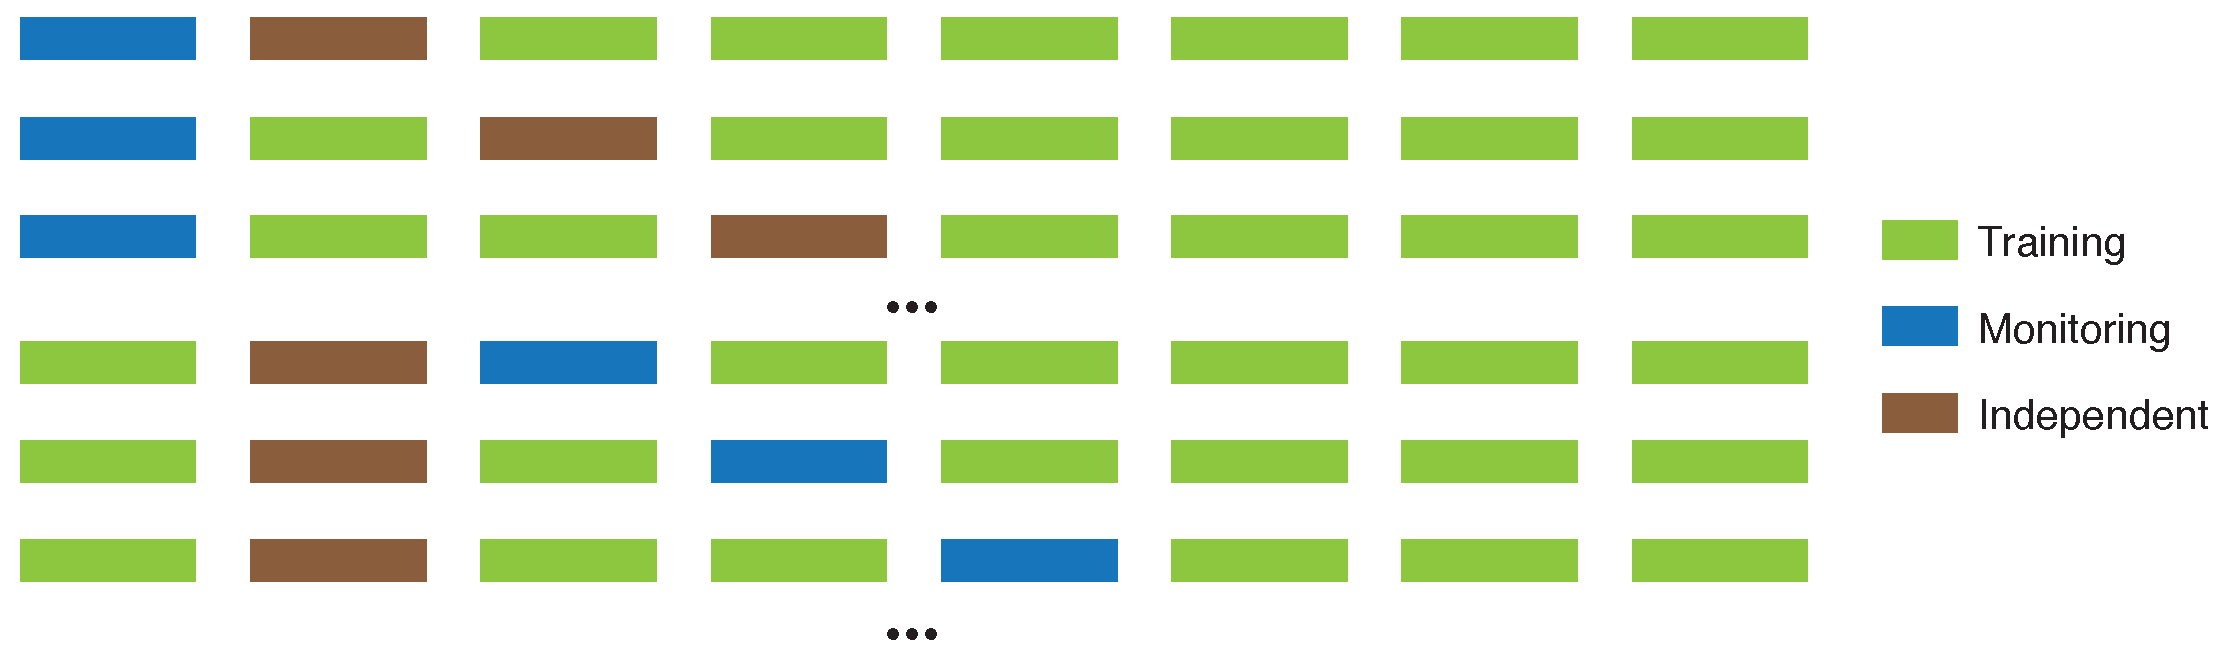
\includegraphics[width=4in]{figures/hts/cross_validation.pdf}
\caption{
A schematic of the cross validation scheme used.
The dataset is partitioned, and sufficient rounds of cross validation are performed such that every block in the partition is used for training, monitoring, and independent validation.
}
\label{fig:crossval_schematic}
\end{figure}

\subsubsection{Network architecture and training}

For the purposes of this study, a feed-forward network with two hidden layers of 100 nodes each was used.
The network was trained using a back-propagation algorithm with network dropout\citep{Hinton:2012tv}.
At each iteration, network dropout disabled 12.5\% of input nodes and 50\% of hidden nodes.
The purpose of network dropout is to prevent the neural network from becoming dependent on the relationships between specific input and hidden nodes in its representation of the model.
This so-called "co-adaptation" can contribute to over-fitting, and thus network dropout makes it possible conduct many more iterations of network training without over-fitting.
The network was trained to classify active and inactive ligands, where activity is measured as log(\ki).
A log(\ki) cutoff of 0.5 was used, and average enrichment was selected as a metric of classification.
Here, we define enrichment as:
\begin{equation}
\label{eq:enrichment}
enrichment = \frac{TP}{TP+FP}/\frac{P}{P+N}
\end{equation}
Where $TP$ and $FP$ are the true positive and false positive rate, $P$ is the total number of positives, and $N$ is the total number of negatives.
Enrichment is typically computed using a cutoff, and average enrichment is computed as the mean enrichment over a range of cutoffs.  In this case the cutoff range used is between 0.0-1.0\% of the total database.
The goal of the average enrichment metric is to have as many true positives as possible relative to false positives within the first 1\% of models selected.
The network is trained for 800 iterations, and the model with the highest average enrichment according to the monitoring data block is selected.

\subsection{Summary of Results}

\subsubsection{Summary of networks trained}
\label{subsubsec:network_training}
Several networks were trained using a variety of input descriptors.
The "Rosetta scalar" network was trained using only the Rosetta generated scalar descriptors in table \ref{table:rosetta_scalar}, the "Rosetta+BCL scalar" network was trained using the Rosetta scalar descriptors combined with the \ac{BCL} descriptors in table \ref{table:bcl_scalar}, and the "Rosetta fingerprint + scalar" network is trained using both the Rosetta scalar, and Rosetta fingerprint descriptors in table\ref{table:rosetta_fingerprint}.
As a control, the "\ac{BCL} scalar" network is trained using only the \ac{BCL} descriptors.
Because the set of training data is balanced in chemical space, we expect that the \ac{BCL} scalar network will not achieve any reasonable enrichment, as no signal should be available for classification.

\subsubsection{Results of network training}

Because the networks described in section \ref{subsubsec:network_training} were trained using a cross-validation scheme, The performance of each of the 90 models generated can be evaluated using the independent dataset for each model.
These independent evaluations were merged to produced a single set of independent predictions spanning the entire training dataset.
These prediction sets were then compared to the classification performance obtained by using the RosettaLigand interface score.
Three prediction performance metrics are presented here: Enrichment (Equation \ref{eq:enrichment}), \ac{PPV} and \ac{ROC-AUC}. 
As described previously, Enrichment provides a metric for the ability of the model to correctly make positive predictions early on.
\ac{ROC} are measurements of the overall performance of the classifier which provide a convenient means of visualizing classification performance. 

\subsubsection{Description of the \acs{ROC-AUC} metric}
To compute an \ac{ROC} curve, the \ac{TPR} is computed as $TPR=TP/P$ where $TP$ is the number of true positive predictions, and $P$ is the number of total positive values in the given dataset, and the \ac{FPR} is computed as $FPR=FP/N$ where $FP$ is the number of false positive predictions, and $N$ is the total number of negative values in the dataset.
The predictions made by each model are sorted by predicted score, with the best scores first, and the \ac{TPR} and \ac{FPR} values are computed for each cumulative fraction of the sorted dataset.
The resulting curve provides a metric of the overall classification performance.
The area under the curve can be computed by integration, resulting in a value between 0.0 and 1.0.
A \ac{ROC-AUC} value of 1.0 indicates a perfect classifier, a value of 0.5 indicates a classifier with a performance equivalent to a coin-toss, and a value of 0.0 indicates a classifier which is always incorrect.

\subsubsection{Description of the \acs{PPV} metric}
\ac{PPV} is a measure of the accuracy of a classifier.  
\ac{PPV} is computed as $PPV=TP/TP+FP$, and can be interpreted as the fraction of positive predictions that are actually positive.
Thus, higher \ac{PPV} indicates a more accurate classifier.

\subsubsection{Summary of classifier performance}
\label{subsubsec:classifier_performance}
The \ac{ROC} and \ac{PPV} metrics can be used to produce a concise visual comparison of the performance of the various networks which were evaluated.
Figure \ref{fig:roc_plot} plots \ac{ROC} curves formed using the networks trained in \ref{subsubsec:network_training}, as well as a classifier which consists entirely of the RosettaLigand interface scores. 
In this experiment, the RosettaLigand interface score based classifier and the "\ac{BCL} Scalar descriptor" network act as controls.
We expect a successful \ac{ANN} to have significant improvement compared to the RosettaLigand interface score classifier, and further that the \ac{BCL} scalar descriptor network have performance roughly equal to a random coin toss.
as shown in the figure, we see that this is the case.  The 3 networks trained using Rosetta interface information all exhibit similar \ac{ROC} curve parameters, all of which are significantly improved over the RosettaLigand interface score classifier.
As expected, the \ac{BCL} scalar descriptor has no classification ability.
Table \ref{table:ann_performance} lists the \ac{ROC-AUC} and average enrichment of each of the plotted classifiers.
We see that the 3 networks trained with RosettaLigand interface score information have similar performance in terms of average enrichment and \ac{AUC}, and that this performance is increased substantially over using only RosettaLigand scoring information for classification.
Specifically, the \ac{ROC-AUC} of the \ac{ANN} classifiers is increased by 0.026-0.036 over the RosettaLigand interface classifier, and the Average Enrichment is increased by 35.93-38.42.
Based on the metrics of \ac{ROC-AUC} and Average enrichment, the three \ac{ANN} models appear to have nearly identical performance.
\begin{figure}
\centering
\includegraphics[width=4in]{figures/hts/tpr_plot.pdf}
\caption{
\acs{ROC} curves showing the performance of the various networks trained using the 507 protein training set.
Performance is plotted using the independent dataset from each of the 90 neural networks used.
The \acs{ROC} curve is plotted as the ratio of \acs{TPR} to \acs{FPR}.
To accentuate the differences in early classification, the X axis is plotted on a log scale.
}
\label{fig:roc_plot}
\end{figure}
\begin{table}
\scriptsize
\renewcommand{\tabcolsep}{0.09cm}
\centering
\begin{tabular}{|c|c|c|}
\hline
Classifier &  Average Enrichment & ROC-AUC \\
\hline
Rosetta Interface scores & 71.66 & 0.891 \\
\hline
ANN: BCL Scalar descriptors & 1.377 & .509 \\
\hline
ANN: Rosetta and BCL Scalar descriptors & 109.62  & 0.927 \\
\hline
ANN: Rosetta Fingerprint and Scalar descriptors & 110.086 & 0.925 \\
\hline
ANN: Rosetta Scalar descriptors & 107.59 & 0.917 \\
\hline
\end{tabular}
\caption{
\acs{ROC-AUC} and average enrichment for the classification models being evaluated.
The Rosetta Interface Scores classifier uses only the sorted RosettaLigand interface scores for classification.
all "\acs{ANN}" classifiers are constructed as neural nets using the specified descriptors.
\acs{ROC-AUC} is the area under the \acs{ROC} curve generated from each descriptor (Figure \ref{fig:roc_plot})
Average enrichment is the average enrichment within the first 1\% of the each dataset.
}
\label{table:ann_performance}
\end{table}

Inspection of the \ac{PPV} of the models, however demonstrates significant performance differences.
Figure \ref{fig:ppv_plot} plots the \ac{PPV} of each model as a function of the \ac{FPR}.
These plots provide a visual depiction of the accuracy of each classifier.
We can see from these models that the models using Rosetta scalar descriptors, or a combination of Rosetta and \ac{BCL} scalar descriptors have siginificantly improved performance relative to the model using Rosetta scalar and fingerprint information.
This suggests that the introduction of fingerprint data results in a loss of model accuracy early in screening.

\begin{figure}
\centering
\includegraphics[width=4in]{figures/hts/ppv_plot.pdf}
\caption{
Plots showing the \acs{PPV} as a function of \acs{FPR} for the various networks trained using the 507 protein training set.
Performance is plotted using the independent dataset from each of the 90 neural networks used.
The \acs{PPV} vs \acs{FPR} curve of an ideal classifier is also plotted, for reference.
To accentuate the differences in early classification, the X axis is plotted on a log scale.
}
\label{fig:ppv_plot}
\end{figure}

\subsubsection{Benchmarking of trained networks using DEKOIS 2.0}
While the performance metrics described in section \ref{subsubsec:classifier_performance} clearly indicate that the \ac{ANN} based classifiers have some value at classifying ligand activity beyond the RosettaLigand interface score and have not been over-trained.
However, the ability of the networks to generalize beyond the training dataset needs to be assessed.
In order to answer the question of whether the \ac{ANN} models demonstrated here are capable of making general predictions, the DEKOIS 2.0 \ref{Bauer:2013de} dataset was used for benchmarking. 
All proteins and ligands were prepared in the same manner as the training data set, and the best scoring model for each protein-ligand complex was selected.
The classifiers previously described were used to re-score the selected protein-ligand complexes, and the \ac{ROC-AUC} for each complex was computed. 
The distribution of \ac{ROC-AUC} across each of the 74 protein-ligand systems is plotted in figure \ref{fig:dekois_roc_all}A.
As expected, the model created using only \ac{BCL} ligand descriptors has no predictive power, and the 3 \ac{ANN} based classifiers have similar, but positive predictive power.
Figure \ref{fig:dekois_roc_all}B shows the Rosetta Fingerprint and scalar model, the RosettaLigand interface score model, and the \ac{BCL} only descriptors.
Closely inspecting this plot, we can see that the primary effect of the Rosetta fingerprint and scalar model (and the other \ac{ANN} classifiers) is to reduce the width of the distribution of \ac{ROC-AUC} scores.  Some highly performing protein targets perform less well, but other targets which are classified worse than random perform better. 

\begin{figure}
\centering
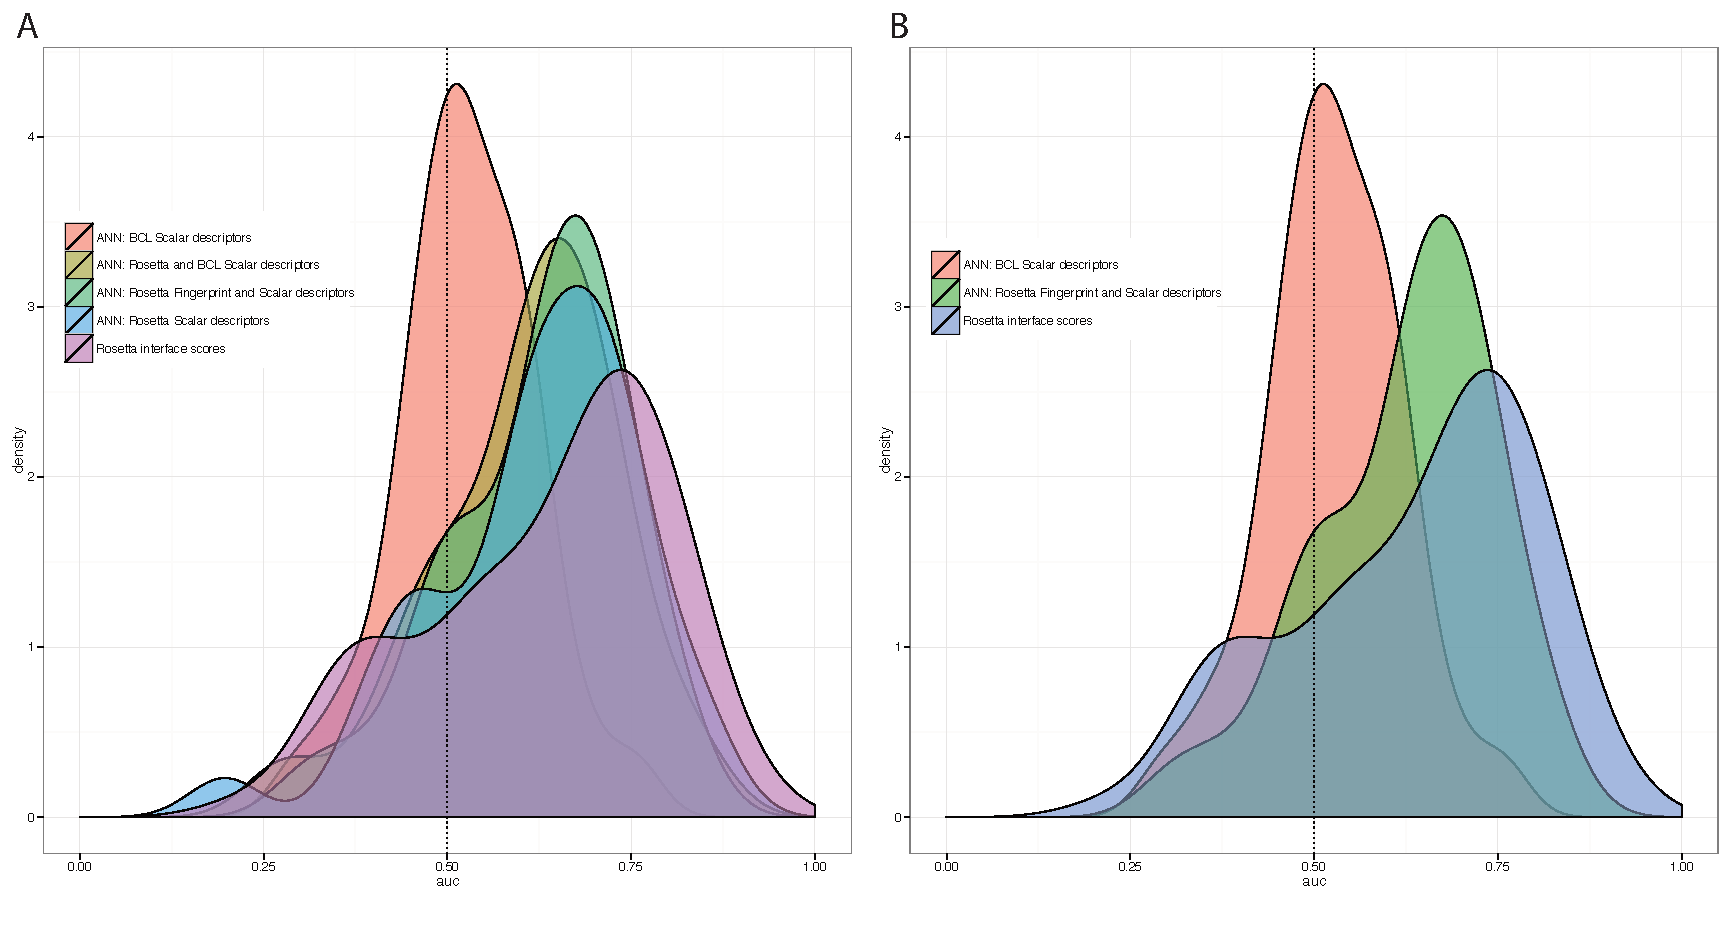
\includegraphics[width=4in]{figures/hts/auc_distributions.pdf}
\caption{
A) A plot of the distribution of \acs{ROC-AUC} values for each of the 74 protein targets in the DEKOIS 2.0 benchmarking set when models were re-scored with each of the classifiers being evaluated.
B) A plot of the distributions for 3 of the evaluated models.
The dotted vertical line indicates the \acs{ROC-AUC} associated with a random model.
\acs{ROC-AUC} values less than 0.5 are worse than random. 
}
\label{fig:dekois_roc_all}
\end{figure}

\section{Discussion}

\subsection{Neural network models can be constructed which improve activity classification over a range of protein and ligand chemical space}

The chemically balanced training data set was successfully used to train \ac{ANN}s to classify ligands based on their binding affinity.
These classifiers were created using a variety of sources of descriptor information, however, based on the cross-validation performance of the \ac{ANN}s trained, it appears that the scalar descriptors generated by RosettaLigand provide the majority of information to the models.
Models trained with a combination of RosettaLigand and \ac{BCL} scalar descriptor information have similar performance to the models trained with RosettaLigand information alone, while models trained with RosettaLigand and Rosetta fingerprint descriptor information seem to be slightly less accurate during early classification.
The former behavior is easily explainable.
It is possible that under certain circumstances, ligand descriptor information may be beneficial to this type of classification model, and that some emergent property might exist between (for example) the flexibility of the ligand and the behavior of that ligand in the RosettaLigand docking simulation.
However, at least in the training dataset used here, there is no evidence for the existence of such an emergent property, and indeed if one does exist it would almost certainly require a dataset comprising a very large range of ligand chemical space to become apparent. 
The loss of accuracy seen upon the addition of the Rosetta fingerprint descriptors suggests that rather than conveying meaningful information about the protein-ligand interface, these descriptors are, instead, introducing noise into the system.
While there is ample historical precedent\citep{Mueller:2010dx,Butkiewicz:2013ka,Hristozov:2007bz} for the value of \ac{RDF} based fingerprint descriptors as \ac{ANN} input, it appears that in this case, the descriptors as implemented are not providing meaningful information.
Regardless, the RosettaLigand based scalar descriptors do provide sufficient information to create a well trained model the performance of which exceeds the performance obtained simply by using the RosettaLigand energy function. 

\subsection{Development of a truly global classifier of protein-ligand binding affinity remains challenging}

Using these models to re-score protein-ligand binding poses indicates that while the models are well trained, they still lack the ability to act generally. Figure \ref{fig:dekois_roc_all} provides some insight into the limits of these models.
When comparing the \ac{ROC-AUC} performance of the neural network models, we see that the width of the distribution of per-system performance narrows.
That is to say, the \ac{ANN} based classifiers tend to perform neither as well nor as poorly as the Rosetta based classifier.
The reduction in the number of systems with \ac{ROC-AUC} significantly worse than random is a highly desirable behavior.
Even a random classifier will return a few true positive results by chance, while a worse than random classifier will be intentionally selecting false positives.
All 3 of the \ac{ANN} based classifiers shown in Figure \ref{fig:dekois_roc_all}A show a decrease in the number of systems with \ac{ROC-AUC} less than 0.4, compared to the Rosetta interface score classifier.
The Rosetta interface score classifier results in 9/72 protein systems with \ac{ROC-AUC} of less than 0.4, while the 3 \ac{ANN} models have only 4/72 protein systems.
Unfortunately, the same effect is observed at the other end of the spectrum.
The Rosetta interface score classifier results in a \ac{ROC-AUC} of 0.75 or higher in 19/72 protein systems, while with the 3 \ac{ANN} models, 7-11 out of 72 protein systems have \ac{ROC-AUC} higher than 0.75. 
One possible cause of the reduced performance is the lack of chemical space covered by the benchmarking set.
The cross-validation performance of the \ac{ANN} based classifiers indicates that the descriptor data used provides sufficient information to improve upon the Rosetta interface score.
However, the 507 ligand set used for this training does not cover the same range of chemical space as the DEKOIS 2.0 benchmark set, and as a result it is likely that in many cases the network is attempting to make predictions far outside of the range of descriptor space that it understands.
While the \ac{ANN} models clearly have classification ability over a large range of the DEKOIS 2.0 dataset, this classification ability is more limited than would be desirable.
The \ac{ANN} models described here demonstrate the possible efficacy of a machine learning approach to structure based virtual screening, however more experimental data is likely required to achieve the goal of a truly general model.
The future directions of this research are outlined in chapter \ref{chap:conclusion}.